\FloatBarrier%
\chapter{Collision SPH}
\label{chap:csph}

We model the collision between elastic solids using a penalty-based contact
force model. A contact force based approach for collision handling will
eliminate the spurious interaction between bodies, which occurs while modeling
with an SPH-based model. The contact force model follows the work of
\textcite{mohseni2021particle}.

The governing equations including the new contact force term are:
\begin{equation}
\label{eqn:sph-continuity}
  \frac{\tilde{d}\rho_a}{dt} = \sum_{b \in A} \; \frac{m_b}{\rho_{b}} \; (
  \rho_{a} \; \tilde{\ten{u}}_{ab} \; + \;
  (\rho \; (\tilde{\ten{u}} \; - \;
  \ten{u}))_{ab}) \; \cdot \nabla_{a} W_{ab}\, ,
\end{equation}
\begin{equation}
\label{eqn:sph-momentum}
  \frac{\tilde{d}\ten{u}_{a}}{dt} = - \sum_{b \in A} m_b \bigg[
  \bigg(\frac{p_a}{\rho_a^2} + \frac{p_b}{\rho_b^2}\bigg) \ten{I} -
  \bigg(\frac{\teng{\sigma}^{'}_{a}}{\rho_a^2} +
  \frac{\teng{\sigma}^{'}_{b}}{\rho_b^2} + \Pi_{ab} \ten{I} \bigg) \bigg]  \cdot \nabla_{a} W_{ab} +
  \ten{g}_{a} + \frac{1}{m_a}\sum_{b \in B} \ten{F}^{\text{cont}}_{a \leftarrow b}.
\end{equation}
Here, $\ten{F}^{cont}_{a}$ is the force acting on particle $a$ due to
\begin{figure}[!htpb]
  \centering
  \includegraphics[width=1.0\textwidth]{images/csph/images/contact_force/contact_force_description}
  \caption{Bodies under collision which are divided into primary and
    secondary.}
\label{fig:bodies_under_collision}
\end{figure}
contact with the other elastic bodies. This is shown in \cref{fig:bodies_under_collision}.

The contact force $\ten{F}^{cont}_{a}$ is computed using
\textcite{mohseni2021particle} formulation. The force acting on a particle $a$
of body A due to the interaction with the particles of body $B$ is into a normal
and tangential component. The normal force $\teng{F}_a^{n}$ on particle $a$ due
to the interaction with the particles $b$ of body $B$ is computed as,
\begin{equation}
  \label{eq:contact-algorithm-normal}
  \ten{F}_a^n = k_r \delta_{n^{c}}^{a} \ten{n}_a^{c}.
\end{equation}
Here, the $\ten{n}_a^{c}$ is a normal vector, and
$\delta_{n^{c}}^{a}$ is an overlap which is computed using a smoothed distance
formulation to handle arbitrarily shaped solids.

Tangential component of the contact force is computed by associating a
tangential spring attached to particle $a$ ($|\Delta \textit{\textbf{l}}_a|$)
and body $B$, which is initiated to a magnitude of zero
($|\Delta \textit{\textbf{l}}_a|=0$). The tangential spring is activated when
the particle comes into contact with body $B$. The tangential force is coupled
to the normal force through the Coulomb's law,
\begin{equation}
  \label{eq:Coulomb-law}
  \ten{F}_{a}^{t} = \min(\mu |\ten{F}_{a}^{n}|, |\ten{F}_{a}^{t}|) \
  \frac{\ten{F}_{a}^{t}}{|\ten{F}_{a}^{t}|}.
\end{equation}
This allows us to impose the sliding friction condition between the
interacting solids.
% =========================================== %
% ------ Results start ---------------------- %
% =========================================== %

\FloatBarrier%
\section{Stress wave propagation in granular media}
\label{sec:results-stress-wave-propagation-with-friction}
% \begin{figure}[!htpb]
%   \centering
%   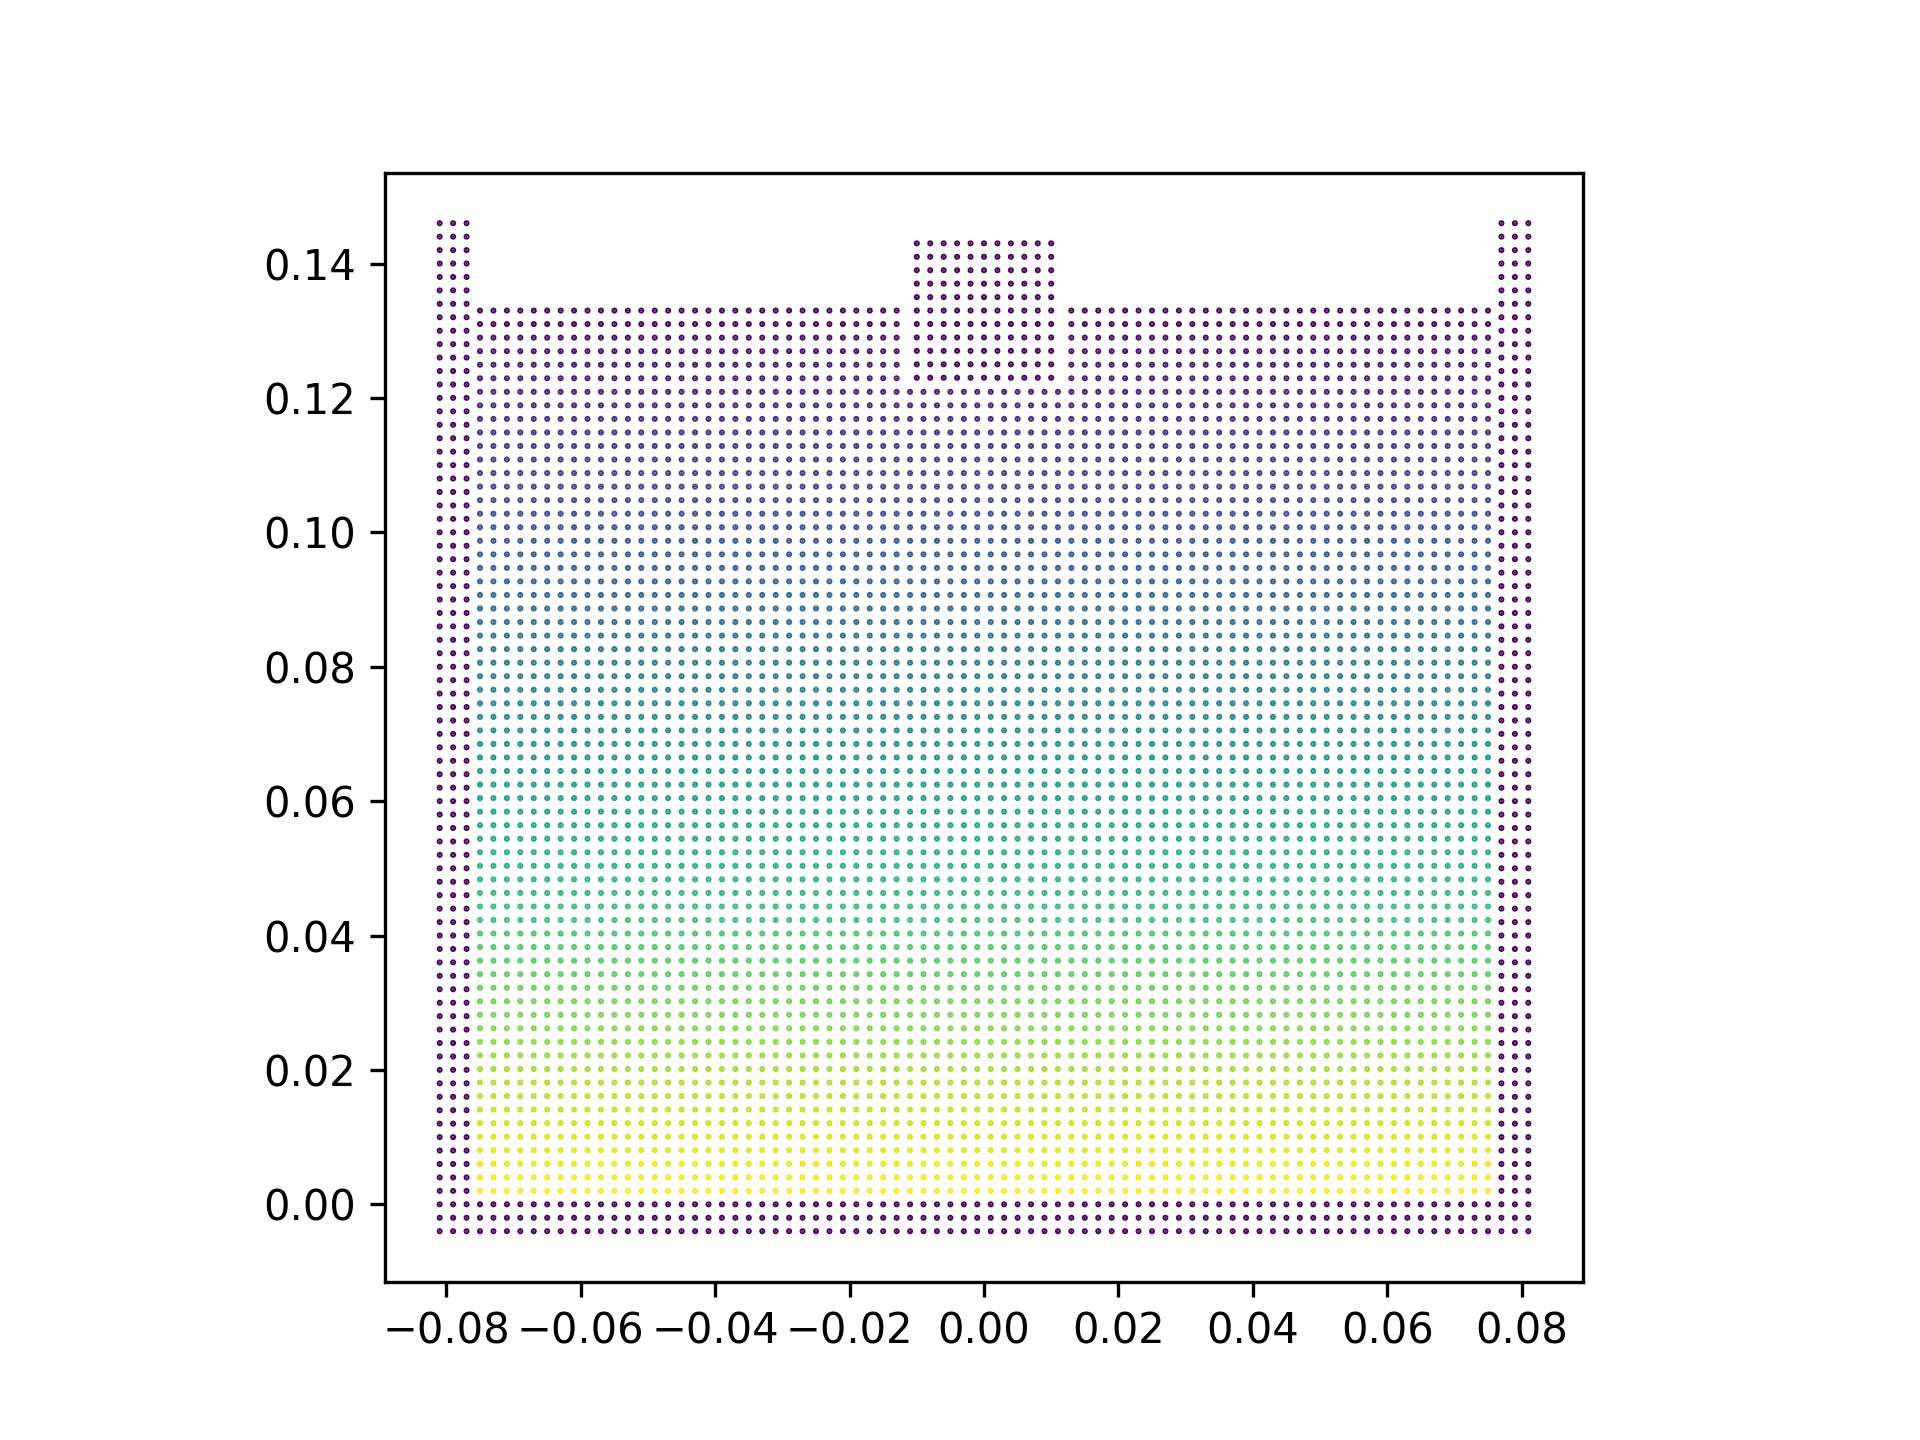
\includegraphics[width=1.0\textwidth]{images/csph/images/de_2021_stress_wave_in_granular_material_part_2/schematic}
%   \caption{Schematic of the initial placement of the frictional granular media including the impactor and walls}
% \label{fig:results-stress-wave-propagation-part-II}
% \end{figure}
We demonstrate in \cref{fig:de-stress-wave-compare}, the current solver abilities in
handling the collision between the multiple elastic solids by simulating the
elastic wave propagation in a granular media. We consider five identical disks
placed at an angle of $45$ degrees, allowed to be impacted by a moving wall from
right with a velocity $5.6$ m\,s\textsuperscript{-1} in horizontal direction.
\begin{figure}[!htpb]
  \centering
  \begin{subfigure}{1.0\textwidth}
    \centering
    \includegraphics[width=0.7\textwidth]{images/csph/images/de_2021_stress_wave_in_granular_material_part_2/bardenhagen_2001}
    \subcaption{}\label{fig:de-stress-wave-bardenhagen}
  \end{subfigure}

  \begin{subfigure}{1.0\textwidth}
    \centering
    \includegraphics[width=0.7\textwidth]{images/csph/images/de_2021_stress_wave_in_granular_material_part_2/tlmpm_2021}
    \subcaption{}\label{}
  \end{subfigure}

  \begin{subfigure}{1.0\textwidth}
    \centering
    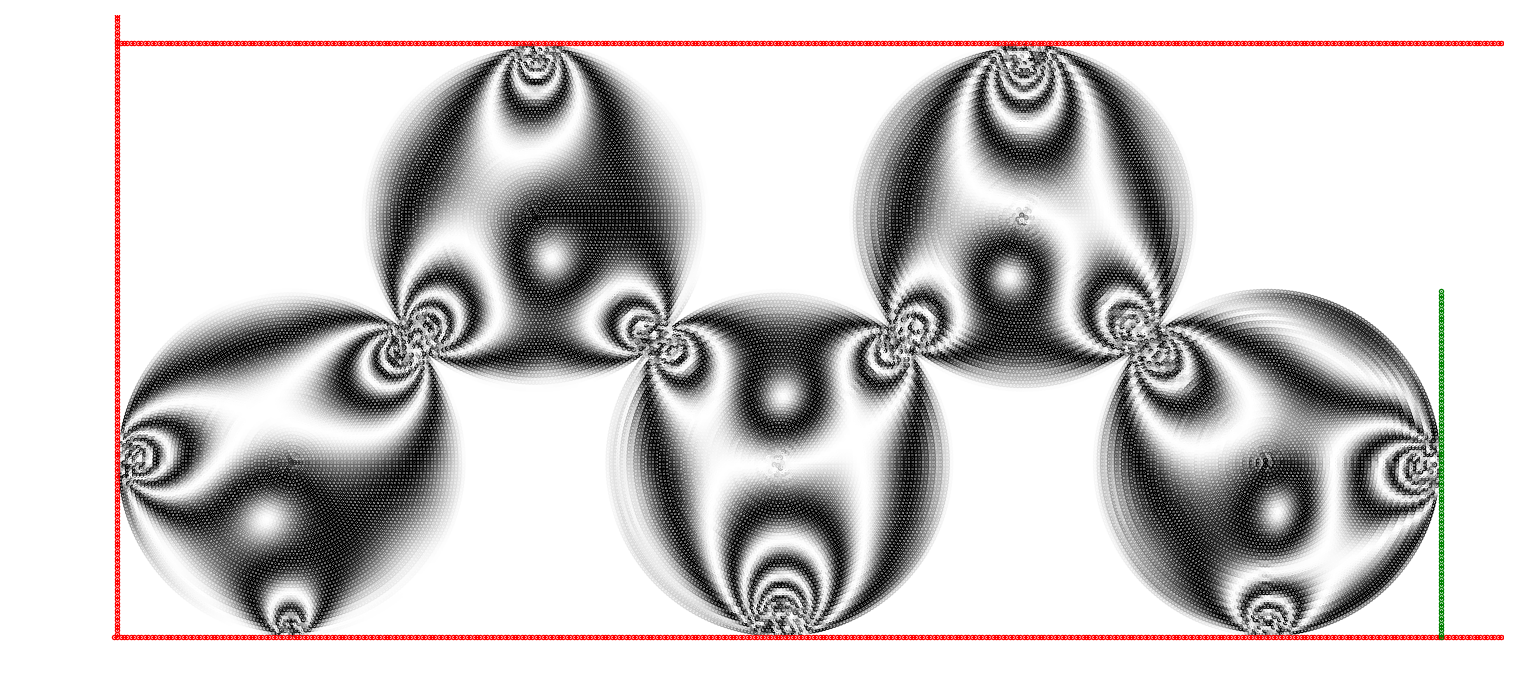
\includegraphics[width=0.8\textwidth]{figures/csph/figures/de_2021_stress_wave_in_granular_material_part_2/case_mohseni/time0}
    \subcaption{}\label{fig:de-stress-wave-current}
  \end{subfigure}
  \caption{Stress fringes of the granular discs from (a) experiment
    \citep{guilkey2001improved}, (b) TLMPM \citep{de2021modelling} (c) Current work}
\label{fig:de-stress-wave-compare}
\end{figure}
